\documentclass[tikz, preview]{standalone}

\usepackage{amsfonts, amsthm, amssymb, amsmath, stmaryrd, etoolbox}
\usepackage{tikz}
\usepackage[all,2cell]{xy}
\usetikzlibrary{matrix,arrows,shapes,decorations.markings,decorations.pathreplacing}
\definecolor{rewritecolor}{rgb}{0,.9,1}
\tikzset{rewritenode/.style={shape=circle,fill=rewritecolor,scale=0.25,font=\Huge}}
\tikzset{RWopen/.style={shape=circle,draw=black,fill=white,scale=0.5,font=\Huge}}
\tikzset{RWclosed/.style={shape=circle,fill=black,scale=0.5,font=\Huge}}
\tikzset{CDnode/.style={shape=circle,fill=white,scale=.5}}
\tikzset{zxgreen/.style={shape=circle,draw,thick,fill=green}}
\tikzset{zxred/.style={shape=circle,draw,thick,fill=red}}
\tikzset{zxyellow/.style={shape=rectangle,draw,thick,fill=yellow}}
\tikzset{zxdiamond/.style={shape=diamond,fill=black,inner sep=2.75}}
\tikzset{zxopen/.style={shape=circle,draw,thick,inner sep=2pt}}
\tikzset{->-/.style={decoration={markings,mark=at position .5 with {\arrow{>}}},postaction={decorate}}}

\begin{document}
\[
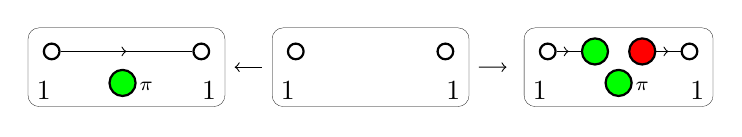
\begin{tikzpicture}
	%
	%
	%
	\begin{scope}[shift={(-5.2,-0.6)}]
	\node [zxgreen,label={[shift={(0.3,-0.4)}]\scriptsize $\pi$}] (v1) at (1.1,-0.3) {};
	\node [zxopen] (v2) at (2.1,0.1) {};
	\node [zxopen] (v3) at (0.2,0.1) {};
	%
	\draw [->-]  (v3) to (v2);
	%
	\node at (0.1,-0.4) {$1$};
	\node at (2.2,-0.4) {$1$};
	\node (v11) at (2.4,-0.1) {};
	\draw [ultra thin, rounded corners] (-0.1,0.4) rectangle (2.4,-0.6);
	\end{scope}
	%
	%
	%
	\begin{scope}[shift={(0.8,-0.1)}]
	\node [zxopen] at (-0.8,-0.4) {};
	\node [zxopen] at (-2.7,-0.4) {};
	%
	\draw [ultra thin, rounded corners] (-3,-0.1) rectangle (-0.5,-1.1);
	\node at (-2.8,-0.9) {$1$};
	\node at (-0.7,-0.9) {$1$};
	\node (v12) at (-3,-0.6) {};
	\node (v14) at (-0.5,-0.6) {};
	\end{scope}
	%
	%
	%
	\begin{scope}[shift={(2.9,-0.8)}]
	
	\node [zxopen] (v1) at (-1.6,0.3) {};
	\node [zxopen] (v2) at (0.2,0.3) {};
	\node [zxgreen] (v4) at (-1,0.3) {};
	\node [zxred] (v5) at (-0.4,0.3) {};
	\node [zxgreen,label={[shift={(0.3,-0.4)}]\scriptsize $\pi$}] (v6) at (-0.7,-0.1) {};
	
	\node at (-1.7,-0.2) {$1$};
	\node at (0.3,-0.2) {$1$};
	%
	\draw [->-]  (v1) to (v4);
	\draw [->-] (v5) to (v2);
	\draw [ultra thin, rounded corners] (-1.9,0.6) rectangle (0.5,-0.4);
	\node (v13) at (-2,0.1) {};
	\end{scope}
	%
	%
	%
	\draw [<-] (v11) edge (v12);
	\draw [<-] (v13) edge (v14);
\end{tikzpicture}
\]
\end{document}
